\chapter{\ifproject%
\ifenglish Project Structure and Methodology\else โครงสร้างและขั้นตอนการทำงาน\fi
\else%
\ifenglish Project Structure\else โครงสร้างของโครงงาน\fi
\fi
}

ในบทนี้จะกล่าวถึงหลักการ และการออกแบบระบบ

\section{หลักการทำงานของแอปพลิเคชัน}
โครงงานนี้เป็นแอปพลิเคชันสำหรับการค้นหาตำแหน่งที่นั่งที่ยังว่างอยู่ภายในสำนักหอสมุดมหาวิทยาลัยเชียงใหม่ พัฒนาขึ้นเป็นรูปแบบเว็บแอปพลิเคชัน
โดยจะ ในส่วนของการวิเคราะห์ได้มีการใช้ Computer Vision และ Machine Learning เข้ามาช่วยในการแยก แล้วนำผลลัพธ์ที่ได้มาคำนวณ แล้วแสดงผลออกมาที่ User Interface
\begin{figure}[h]
\centering
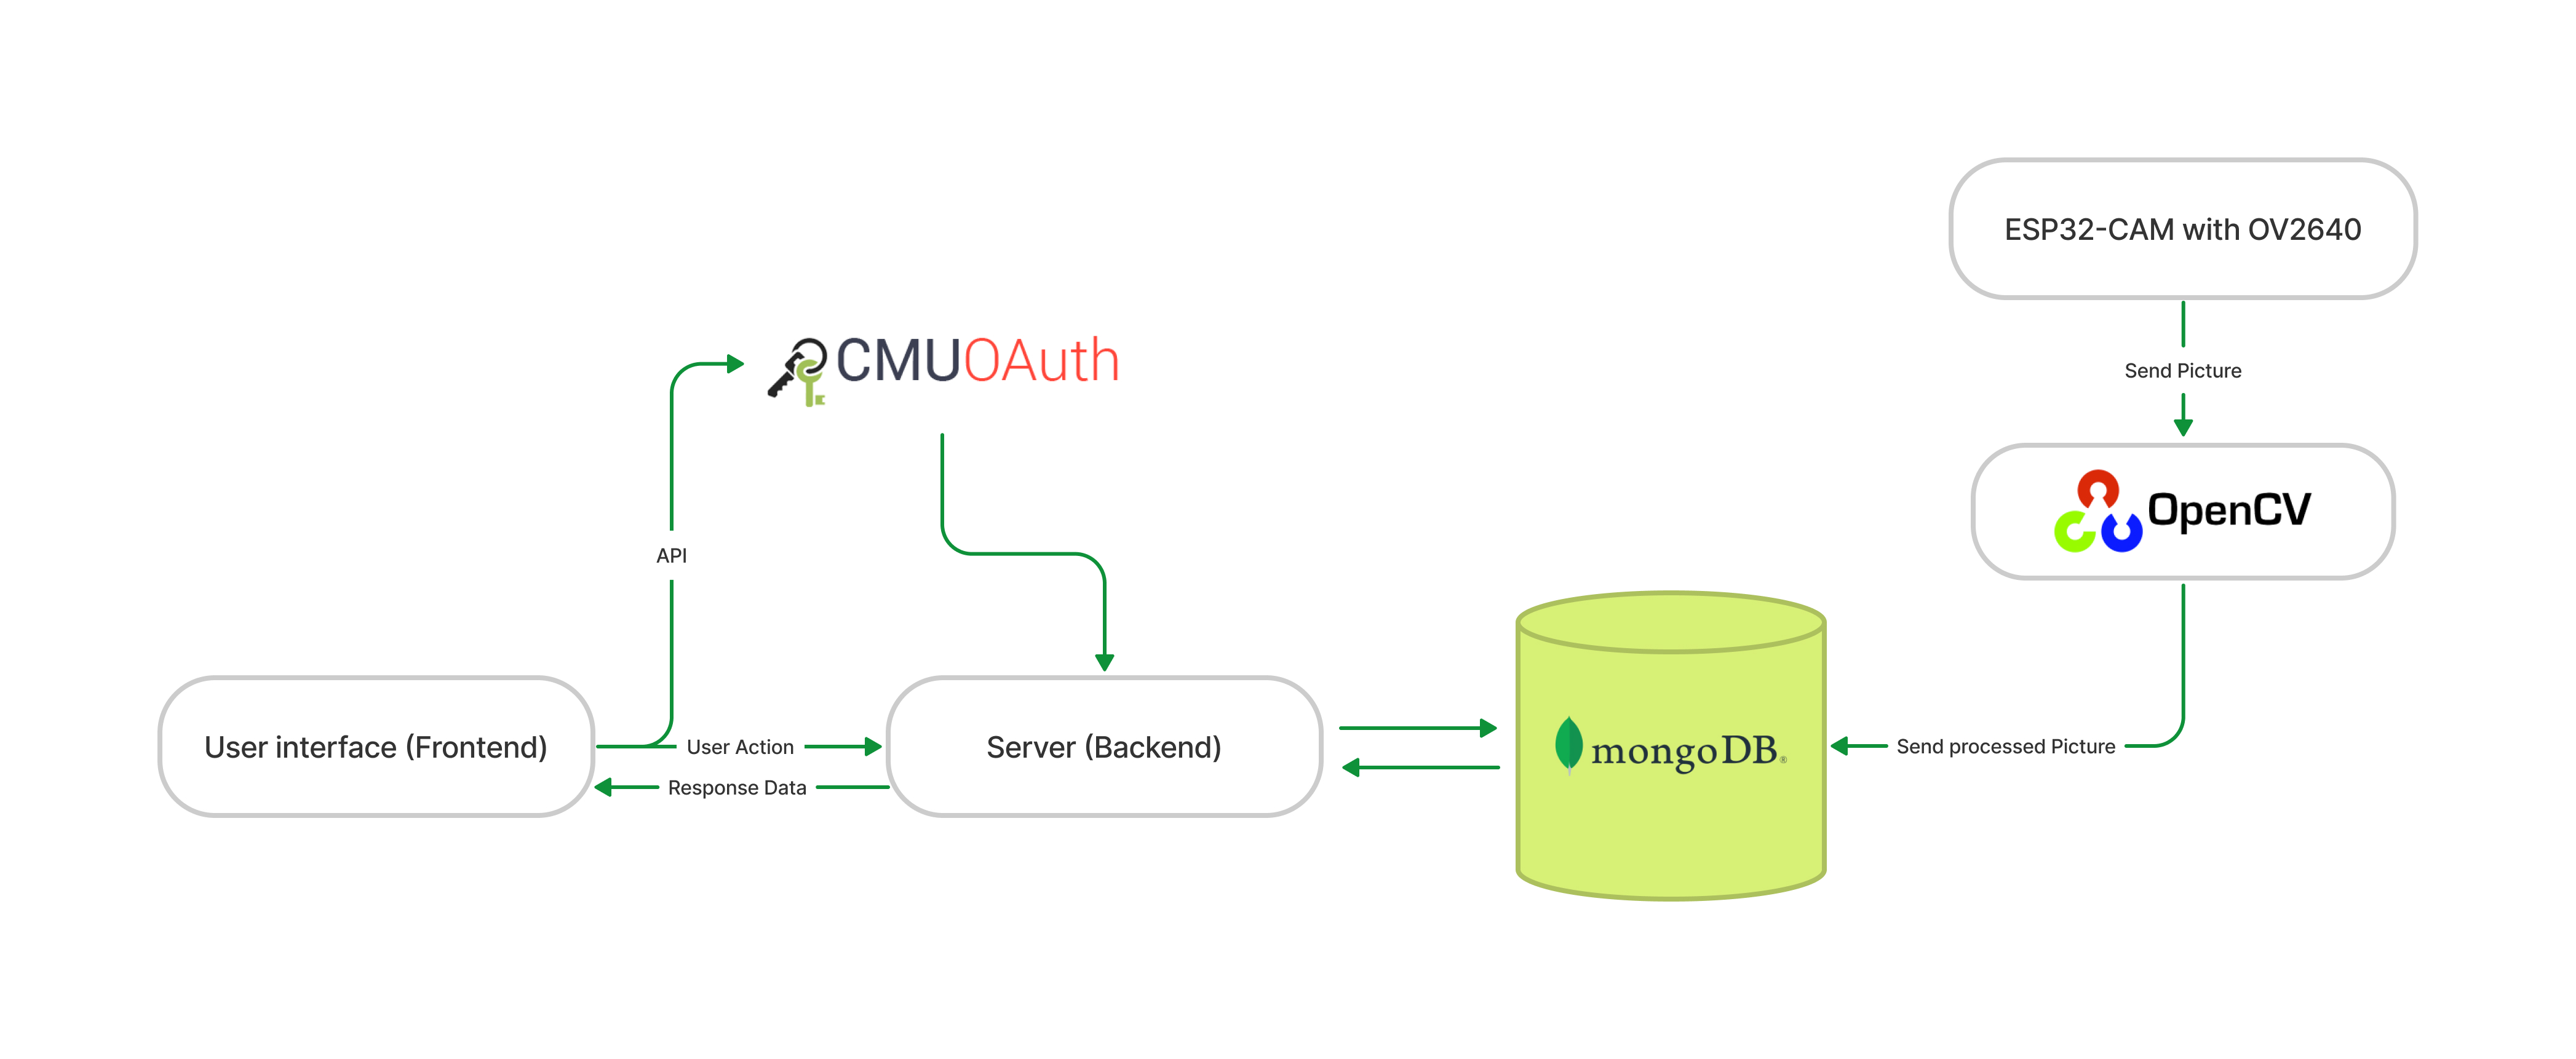
\includegraphics[width=\textwidth]{System Diagram.jpg}
\caption[System Overview]{System Overview}
\label{fig:System}
\end{figure}

\section{การใช้งานของแอปพลิเคชัน}
\subsection{ผู้ใช้ทั่วไป}
\subsection{นักศึกษาและบุคลากรในมหาวิทยาลัย}
\subsection{หอสมุด}